
% -> Seleção das atas
% -> Seleção dos anotadores
% -> Processo para geração das atas de referência
% -> Imagem das concordâncias.
% -> Mostrar a segmentação de referência como resultado

Falar como deve ser o processo de anotação conforme feito por Holy...

 % \subsubsection{Avaliação dos Segmentadores}
 %  Critérios de avaliação
A avaliação de um segmentador automático de textos exige uma referência, isto é, um texto com os limites entre os segmentos conhecidos. Essa referência, deve ser confiável, sendo uma segmentação legítima que é capaz de dividir o texto em porções relativamente independentes, ou seja, uma segmentação ideal.

% ->------> Seleção das atas
Para isso, selecionou-se um conjunto de atas reais coletadas do Departamento de Computação da UFSCar campus Sorocaba. Analisou-se as atas públicas das reuniões do Conselho de Pós-Graduação e Conselho de Graduação desse departamento das quais foram selecionadas seis atas de cada conselho, sendo cinco referentes a reuniões ordinária e uma reunião extraordinária, totalizando doze documentos. Esses documentos foram escolhidos de forma que o conjunto final contenha atas com tamanhos diferentes (entre 1 e 4 páginas), e maior diversidade de conteúdo.
 % contém tabelas e listas

Em seguida, selecionou-se um grupo de anotadores para analisar e coletar dados referentes a segmentação de cada ata. O grupo de anotadores foi formado por profissionais com alguma afinidade com atas de reunião, como profissionais administrativos, professores e coordenadores de curso. Optou-se por utilizar um \textit{software} como ferramenta para a coleta dos dados a fim de facilitar o trabalho de anotação e diminuir eventuais erros, conforme sugerido por~\cite{}. Essa ferramenta permitiu aos anotadores visualizar os documentos e indicar livremente as divisões entre segmentos, bem como rotulá-los em classes e indicar palavras que melhor descrevem o assunto central do segmento.
Os anotadores receberam informações básicas sobre o objetivo da pesquisa e instruções de como operar o \textit{software}. Contudo, nenhum critério foi estabelecido para o procedimento ficando os anotadores livres para segmentar e rotular as atas orientados apenas pela interface da ferramenta. Na Figura~\ref{fig:interfaceanotacoes} é mostrada a interface da ferramenta utilizada para as anotações.

  \begin{figure}[!h]
	  \centering
	  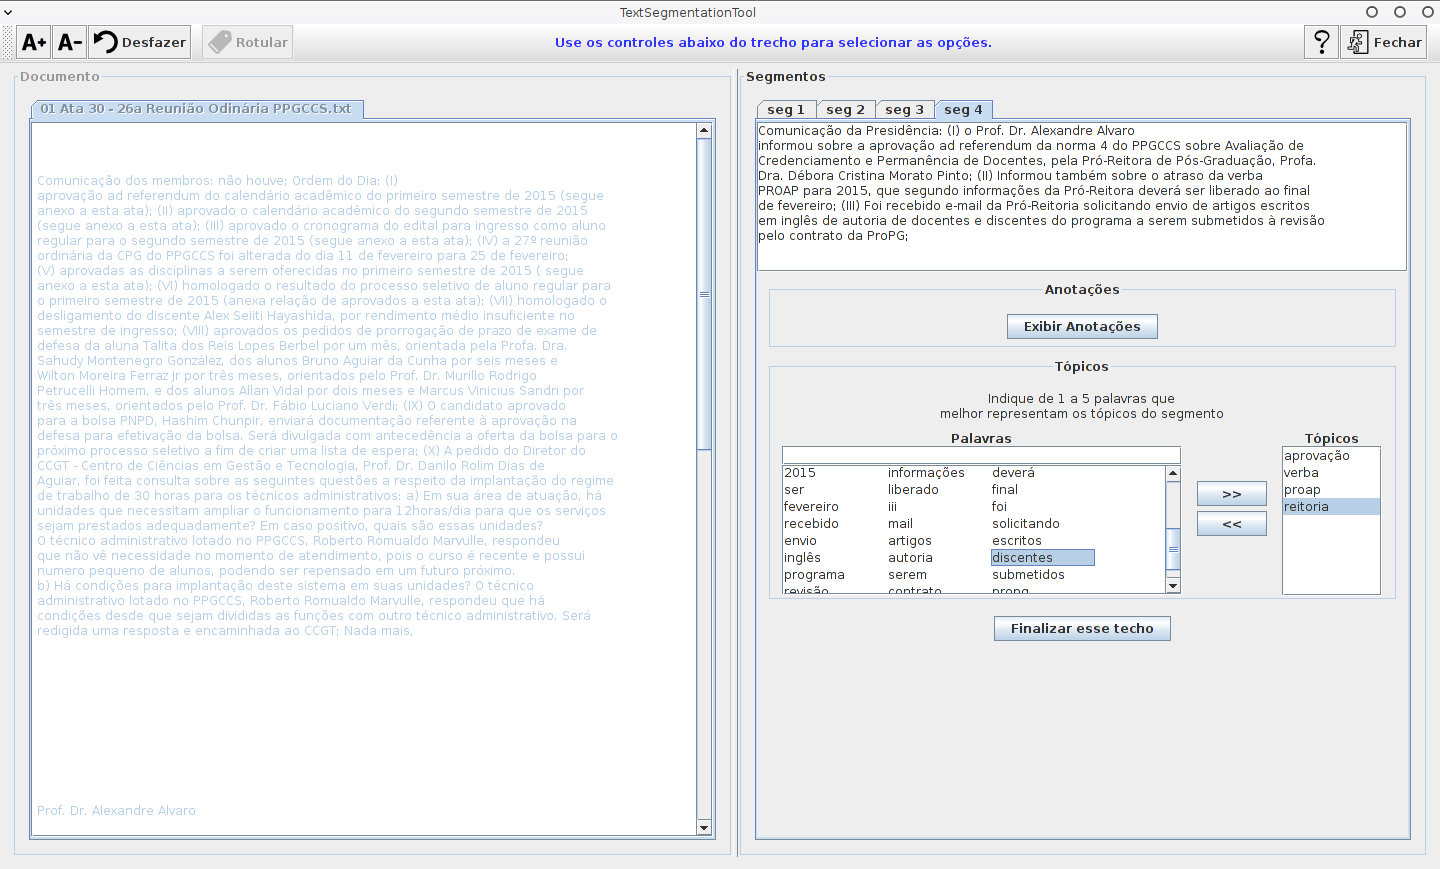
\includegraphics[width=0.9\paperwidth]{conteudo/capitulos/figs/interface-anotacoes.png}
	  \caption{Interface da ferramenta utilizada para anotações onde o texto a ser segmentado é exibido no painel a esquerda e os controles para anotação estão disponíveis a direita}
	  \label{fig:interfaceanotacoes}
  \end{figure}


--> falar que foi usado maior concordânica igual feio por Hearts.
  
Após o processo de anotação, os dados coletados foram analisados para gerar as segmentações de referência. Considerou-se que





% ->----------------------------------------------------------------------------------

  Para isso, utilizou-se um \textit{software}, desenvolvido com esse objetivo especifico, que permitiu aos anotadores visualizar um documento, e indicar livremente as divisões entre segmentos. 

%%%%%%%%%%%	
	03 Ata 36 - 31a Reunião Odinária PPGCCS.txt.csv
	0 0 0 1 0 0 0 0 1 0 0 0 0 0 0 0 0 0 0 1 1 0 0 0 1 0 
	1 0 0 1 0 1 1 1 1 1 0 0 0 1 0 1 1 1 1 1 1 0 0 1 1 0 
	0 0 0 1 0 0 0 0 1 0 0 0 0 0 1 1 0 1 0 1 1 0 0 1 1 0 
	0 0 0 1 0 1 1 0 1 1 1 0 0 1 0 1 0 1 0 1 1 0 0 1 1 0 
	----------------------------------------------------
	0 0 0 1 0 0 0 0 1 0 0 0 0 0 0 1 0 1 0 1 1 0 0 1 1 0 
	-->./SegReferences/03 Ata 36 - 31a Reunião Odinária PPGCCS.txt.csv
%%%%%%%%%%%	




%%%%%%%%%%%	

12 Nomes de Aquivos de referência

01 Ata 30 - 26a Reunião Odinária PPGCCS.txt.csv
	Anotador N   7 segmetnos |  25 sentenças
	Anotador N  15 segmetnos |  25 sentenças
	Anotador N   8 segmetnos |  25 sentenças
	Anotador N  16 segmetnos |  25 sentenças
02 Ata 29 - 25a Reunião Odinária PPGCCS.txt.csv
	Anotador N   4 segmetnos |  17 sentenças
	Anotador N  14 segmetnos |  17 sentenças
	Anotador N   6 segmetnos |  17 sentenças
	Anotador N  14 segmetnos |  17 sentenças
03 Ata 36 - 31a Reunião Odinária PPGCCS.txt.csv
	Anotador N   6 segmetnos |  26 sentenças
	Anotador N  17 segmetnos |  26 sentenças
	Anotador N  10 segmetnos |  26 sentenças
	Anotador N  14 segmetnos |  26 sentenças
04 Ata 32 - 28a Reunião Odinária PPGCCS.txt.csv
	Anotador N   5 segmetnos |  26 sentenças
	Anotador N  12 segmetnos |  26 sentenças
	Anotador N   7 segmetnos |  26 sentenças
	Anotador N  12 segmetnos |  26 sentenças
05 Ata 33 - 29a Reunião Odinária PPGCCS.txt.csv
	Anotador N   4 segmetnos |  33 sentenças
	Anotador N  17 segmetnos |  33 sentenças
	Anotador N   9 segmetnos |  33 sentenças
	Anotador N  16 segmetnos |  33 sentenças
06 Ata 35 - 5a Reunião Extraodinária PPGCCS.txt.csv
	Anotador N   3 segmetnos |  11 sentenças
	Anotador N   9 segmetnos |  11 sentenças
	Anotador N   4 segmetnos |  11 sentenças
	Anotador N   5 segmetnos |  11 sentenças
07 20ª Reunião Extraordinária CoC-CCS 08-12-10.txt.csv
	Anotador N   3 segmetnos |  20 sentenças
	Anotador N   5 segmetnos |  20 sentenças
	Anotador N   4 segmetnos |  20 sentenças
08 25ª Reunião Ordinária CoC-CCS 04-04-12.txt.csv
	Anotador N   4 segmetnos |  35 sentenças
	Anotador N   5 segmetnos |  35 sentenças
	Anotador N   9 segmetnos |  35 sentenças
09 40ª Reunião Ordinária CoC-CCS 06-05-15.txt.csv
	Anotador N   3 segmetnos |  24 sentenças
	Anotador N   3 segmetnos |  24 sentenças
	Anotador N   9 segmetnos |  24 sentenças
10 20ª Reunião Ordinária CoC-CCS 01-06-11.txt.csv
	Anotador N   4 segmetnos |  50 sentenças
	Anotador N   5 segmetnos |  50 sentenças
	Anotador N   8 segmetnos |  50 sentenças
11 10ª Reunião Ordinária CoC-CCS 05-04-10.txt.csv
	Anotador N   4 segmetnos |  43 sentenças
	Anotador N   5 segmetnos |  43 sentenças
	Anotador N  12 segmetnos |  43 sentenças
12 13ª Reunião Ordinária CoC-CCS 05-08-10.txt.csv
	Anotador N   3 segmetnos |  56 sentenças
	Anotador N   4 segmetnos |  56 sentenças
	Anotador N  11 segmetnos |  56 sentenças


%%%%%%%%%%%	










Como foram obtidas (software e especialistas) 
A fim de obter um conjunto de documentos segmentados que possam servir como referência na avaliação, os documentos coletados foram segmentados manualmente por dois coordenadores de curso que participam de reuniões. 


Com o uso desse \textit{software} foram coletados os dados de seis atas segmentadas pelos participantes das reuniões, os quais serviram como referência para a avaliação dos algoritmos. O \textit{software} desenvolvido para segmentação manual está disponível para utilização e consulta em~\urlsoftwares	

Os arquivos gerados foram tratados para que os segmentos sempre terminem em uma sentença reconhecida pelo algoritmo, uma vez que as sentenças são a unidade mínima de informação nesse trabalho.

A Tabela~\ref{tab:segmentacaoreferencia} contém, para cada ata, a quantidade de sentenças e a quantidade de segmentos identificadas pelos participantes.


% Referência ····························································
% Documento	|	Segmentos Esp 1 |	Segmentos Esp 2
% Doc1		|	7 				|	15
% Doc2		|	9 				|	20
% Doc3		|	7 				|	15
% Doc4		|	9 				|	17
% Doc5		|	4 				|	9 
% Doc6		|	11				|	17
\begin{table}[!h]
	\centering
	\begin{tabular}{|l|c|c|c|} \hline
		\textbf{Ata} & \textbf{Sentenças}  & 
		\textbf{Participante 1}  & 
		\textbf{Participante 2} \\	\hline

		Ata 1 & 18 & 7  & 15 \\ \hline 
		Ata 2 & 26 & 9  & 20 \\ \hline 
		Ata 3 & 24 & 7  & 15 \\ \hline 
		Ata 4 & 32 & 9  & 17 \\ \hline 
		Ata 5 & 25 & 11 & 17 \\ \hline 
		Ata 6 & 10 & 4  & 9  \\ \hline 

	\end{tabular}
	\caption{Quantidade de sentenças e segmentos de referência por ata.}
	\label{tab:segmentacaoreferencia}
\end{table}
























% Obtem-se nesse cenário uma eficiência maior em relação a segmentação da ata, o que sugere que textos mais estruturados podem ter melhores benefícios com essa técnica e que as atas possuem menor coesão léxica em comparação à textos organizados em seções.  % ou a premissa do algoritmo não é tão boa.




\subsection{Configuração experimental}
\label{subsec:configuracaoexperimental}

%%%%%%%%%%%%%%%%%%%%%%%%%%%%%%%%%%
% Falar dos parametros do TT
% falar dos testes e qual foi a melhor configuração.
% mostrar um gráfico com essa configuração.
% mostrar o gráfico dos generos musicais.
% 
% De certa forma, tratar o C99 e o TT como pertencentes a mesma técnica = coesão léxica!!
% e depois justificar o por que de usar outras técnicas
%%%%%%%%%%%%%%%%%%%%%%%%%%%%%%%%%%




  
% --> Falar da coesão léxica peculiar das atas!!



























A seguir...

Antes de ...



	





% \begin{tabular}{|l|c|c|c|c|c|c|c|} 
% \hline 
% M\'{e}todo    &  \textbf{Pk}   & \textbf{WD}    & \textbf{A }    & \textbf{P } & \textbf{R } & \textbf{F1} & \textbf{SG}\\ \hline
% Senten\c{c}as & 0.320          & 0.502 & 0.498 & 0.498 & \textbf{1.000} & \textbf{0.642} & 22.083\\ \hline
% TextTiling    & 0.275          & 0.469 & 0.531 & 0.514 & 0.937 & 0.640 & 19.583\\ \hline
% C99           & 0.142          & 0.426 & 0.574 & 0.601 & 0.473 & 0.506 & 8.167\\ \hline
% BayesSeg      & 0.148 & 0.414 & 0.586 & 0.599 & 0.526 & 0.528 & 8.750\\ \hline
% MinCut        & 0.226  & 0.532          & 0.468 & 0.464 & 0.438 & 0.432 & 10.333\\ \hline
% TextSeg       & \textbf{0.085} & \textbf{0.387} & \textbf{0.613} & \textbf{0.714} & 0.412 & 0.497 & 5.167\\ \hline
% \end{tabular} 




%  Remoção de termos
% \item Redução de termos: algumas palavras irrelevantes que não contribuem para a distinção do texto em tópicos ou categorias devem ser removidas, como artigos, preposições, pronomes, verbos de estado\footnote{Apresentam uma situação inativa, onde o verbo não expressa uma alteração, mas apenas uma propriedade ou condição dos envolvidos.}. 
% ARRUMAR -------------------------------------
	% Trata-se também \textit{stop words} as palavras de uso muito frequente dentro de um determinado domínio as quais não são capazes de discriminar documentos, portanto também não devem fazer parte dos atributos~\cite{Rezende2003}. Essas palavras são chamadas de \textit{stopwords}. 



% O módulo de preparação e manutenção recebe uma coleção de documentos e produz uma estrutura de dados interna, que é utilizada pelo módulo de consulta, que por sua vez, é responsável por receber a intensão usuário, proceder a busca na estrutura de dados interna e retornar os trechos associados com a intensão do usuário, tanto quanto ao assunto como no tipo de ocorrência. A Figura \ref{fig:visao-geral} mostra a visão geral do sistema com suas principais entradas e saídas. 


% O objetivo do sistema é permitir ao usuário consultar uma coleção de documentos de reuniões a fim de obter todo o histórico de ocorrências de um determinado tema pesquisado, podendo identificar nos documentos onde o tema foi mencionado como informe ou onde houve uma decisão sobre o tema. Para isso, o sistema é divido em dois módulos principais: Módulo de preparação e manutenção e Módulo de consulta.






 
% Um cabeçalho é a porção de texto que inicia cada página do documento e se repete ao longo do texto, de forma semelhante, um rodapé encerra as páginas. 
	% Um cabeçalho é a porção de texto inicial de documento que se repete ao longo do texto, da mesma forma um rodapé se repete. Detecta-se um cabeçalho sempre que há uma repetição das primeiras palavras do documento.

% ==========| Stop words |==========



% verbo inativo --> http://www.lpeu.com.br/q/sj8n2

% Redução de termos: eliminou-se as \textit{stop words} por meio de uma lista de 438 palavras. Além disso, eliminou-se a acentuação, sinais de pontuação, numerais e todos os \textit{tokens} menores que três caracteres. 















o módulo de preparação/manutenção recebe como entrada os documentos que compõe a base de consultas e produz uma estrutura de dados interna que será utilizada pelo módulo de consulta. Resumidamente, divide cada documento em segmentos de texto, que contêm um assunto predominante. Em seguida cada segmento será classificado de acordo o tipo da ocorrência de cada assunto, que pode ser, por exemplo, uma decisão ou um informe. Assim, a estrutura de dados interna registrará quais assuntos foram tratados na reunião, bem como o trecho do documento onde é discutido e seu tipo. Os tipos de ocorrência, que serão tratadas pelo sistema, serão ainda estabelecidos em conjunto com usuários especialistas, com base em uma amostra de documentos.

Uma vez que os segmentos estejam rotulados e representados computacionalmente, a tarefa é identificar qual assunto está presente em cada trecho e qual é o tipo de ocorrência. A fim de encontrar o principal assunto abordado em um trecho, pretende-se usar uma ferramenta de extração de tópicos para produzir uma base de trecho/tópicos, a qual será parte da estrutura de dados interna.

Essa estrutura irá descrever cada segmento de texto. Essa descrição irá conter, para cada segmento, dados do documento do qual foi extraído, bem como seus rótulos que indicarão o tipo da ocorrência e os tópicos que são tratados nesse fragmento de documento.

De maneira geral, esse módulo divide cada documento em segmentos de texto, que contêm um assunto predominante. 


Em seguida cada segmento será classificado de acordo o tipo da ocorrência de cada assunto, que pode ser, por exemplo, uma decisão ou um informe. Assim, a estrutura de dados interna registrará quais assuntos foram tratados na reunião, bem como o trecho do documento onde é discutido e seu tipo. Os tipos de ocorrência, que serão tratadas pelo sistema, serão ainda estabelecidos em conjunto com usuários especialistas, com base em uma amostra de documentos.



% O módulo de preparação e manutenção, tem como funções principais, 
% receber as atas, extrair e segmentar o texto, realizar o pré-processamento,  produzir uma representação matricial dos segmentos das atas originais, modelar um classificador/extrair os tópicos e entregar ao módulo de consulta a estrutura de dados interna. 


















Entre os principais trabalhos da literatura podemos citar o  \textit{TextTiling}~\cite{Hearst1994} e o \textit{C99}~\cite{Choi2000}.
%
%%%%%%%%%%%%%%%%%%%%%%%%%%%%%%%%%%%%%%%%%%%%%%%
%%%              TextTiling                 %%%
%%%%%%%%%%%%%%%%%%%%%%%%%%%%%%%%%%%%%%%%%%%%%%%
O \textit{TextTiling} é um algoritmo baseado em janelas deslizantes, em  que, para cada candidato a limite, analisa-se o texto circundante. Um limite ou quebra de segmento é identificado sempre que a similaridade cai abaixo de um limiar.
% \textit{threshold}. %TODO - explicar como se encontra os vales


O \textit{TextTiling} recebe uma lista de candidatos a limite, usualmente finais de parágrafo ou finais de sentenças. Para cada posição candidata são construídos 2 blocos, um contendo sentenças que a precedem e outro com as que a sucedem. O tamanho desses blocos é um parâmetro a ser fornecido ao algoritmo e determina o tamanho mínimo de um segmento.
%
Em seguida, os blocos de texto são representados por vetores que contém as frequências de suas palavras. Então, usa-se cosseno (Equação~\ref{equ:cosine}) para calcular a similaridade entre os blocos adjacentes a cada candidato e identifica-se uma transição entre tópicos pelos vales na curva de dissimilaridade.

%TODO como apresentado na Figura~\ref{fig:curvadedissimilaridade}.


O \textit{TextTiling} possui baixa complexidade computacional. Por outro lado, algoritmos mais complexos, como os baseados em matrizes de similaridade, apresentam acurácia relativamente superior como apresentado em~\cite{Choi2000, Kern2009, Misra2009}.

%%%%%%%%%%%%%%%%%%%%%%%%%%%%%%%%%%%%%%%%%%%%%%%
%%%                  C99                    %%%
%%%%%%%%%%%%%%%%%%%%%%%%%%%%%%%%%%%%%%%%%%%%%%%

O C99 é um algoritmo baseado em ranking.
% Choi \cite{Choi2000} apresenta um algoritmo baseado em ranking, o \textit{C99}. 
%
Embora muitos trabalhos utilizem matrizes de similaridades para pequenos segmentos, o cálculo de suas similaridades não é confiável, pois uma ocorrência adicional de uma palavra causa um impacto que pode alterar significativamente o cálculo da similaridade~\cite{Choi2000}.
%
Além disso, o estilo da escrita pode não ser constante em todo o texto. Por exemplo, textos iniciais dedicados a introdução costumam apresentar menor coesão do que trechos dedicados a um tópico específico. Portanto, comparar a similaridade entre trechos de diferentes regiões não é apropriado.
% Complexidade O(n²)
Devido a isso, as similaridades não podem ser comparadas em valores absolutos. Então, contorna-se esse problema fazendo uso de \textit{rankings} de similaridade para encontrar os segmentos de texto. 


Inicialmente é construída uma matriz que contém as similaridades de todas as unidades de texto. Em seguida, cada valor na matriz de similaridade é substituído por seu ranking local. Para cada elemento da matriz, seu \textit{ranking} é o número de elementos vizinhos com valor de similaridade menor que o seu.
% O que é a máscara
Então, cada elemento e comparado com seus vizinhos dentro de uma região denominada máscara.
%

Na Figura~\ref{fig:a} é destacado um quadro 3~x~3 de uma matriz em que cada elemento é a similaridade entre duas unidades de informação. 
%
Tomando como exemplo o elemento com valor $0,5$, a mesma posição na matriz de \textit{rankings} terá o valor $4$, pois esse é o número de vizinhos com valores inferiores a $0,5$ dentro do quadro analisado na matriz de similaridades. Da mesma forma, na Figura~\ref{fig:b} para o valor $0,2$ a matriz de \textit{rankings} conterá o valor $1$ na mesma posição.









% ----------------------------------------------------------------------------- 


% O \textit{TextTiling} obteve o melhor desempenho em revocação, utilizando-se janelas de tamanho igual a $20$ e passo igual a $3$, onde registrou-se uma média de $0,917$ para essa medida.
%
%
%Embora haja melhora de desempenho com os valores apresentados, os testes apontam que não há diferença significativa de performance entre as configurações. O pré-processamento é capaz de reduzir o tamanho do texto mantendo a qualidade final dos algoritmos, sobre tudo em textos longos e grandes coleções de documentos.
%
%
%%%%%%%%%%
% Definição do que é um bom algoritmo de segmentação
%%%%%%%%%%
%Para fins de avaliação desse trabalho, um bom método de segmentação é aquele cujo resultado melhor se aproxima de uma segmentação manual, sem a obrigatoriedade de estar perfeitamente alinhado com tal. 
%
%
%
%Dado o contexto das atas de reunião, e a subjetividade da tarefa de segmentação, não é necessário que os limites entre os segmentos (real e hipótese) sejam idênticos, mas que se assemelhem em localização e quantidade.
% 
%
%Nesse sentido, 


% Desempenho dos métodos 
% 
% C99 é um pouco melhor mas tem mais complexidade
% 



% Na maioria das medidas, o algoritmo \textit{C99} sobressaiu-se em relação ao \textit{TextTiling}, contudo, testes estatísticos realizados indicaram que não houve diferença significativa. 

%%%%%%%%%%%%%%%
% O Impacto do Preprocessamento 
%%%%%%%%%%%%%%%
%Da mesma forma, a etapa de preprocessamento proporciona melhora de performance quando aplicada, porém o seu maior benefício é a diminuição do custo computacional, uma vez que não prejudica a qualidade dos resultados.



%Em ambos os algoritmos os parâmetros que mais influenciam na quantidade de segmentos extraídos são para o \textit{TextTiling} o tamanho da janela e para o \textit{C99} a proporção de segmentos em relação a quantidade de candidatos. Observa-se que a quantidade de segmentos automáticos melhora os resultados principalmente e P$_k$ e \textit{WindowDiff}. 


%Melhores resultados foram percebidos quando os algoritmos aproximam a quantidade de segmentos automáticos da quantidade de segmentos da referência. Embora os parâmetros \textit{S} e \textit{J} influenciem na quantidade de segmentos extraídos, não se conhece a 

%melhores resultados de foram percebido com X e Y segmntos extraidos
%
%o que reforça o 
%
%Contudo, não possível conhecer esses valores e o parâmetros baseiam-se na quantidade de candidatos e 
%
%O parâmetro \textit{J} influência diretamente 
%
%
%
%A quantidade de segmentos extraídos
%
%A configuração da proporção de segmentos em relação ao número de candidatos (S) influencia diretamente n
%
%

%
%a quantidade de segmentos de referência é subjetiva


%e Precisão melhores resultados quando retorna-se menos segmentos o que pode ser explica 
%
%Contudo, não possível conhecer esses valores e o parâmetros baseiam-se na quantidade de candidatos e 

%Os resultados indicam que os algoritmos apresentam desempenho similar a outros trabalhos~\cite{arabi} 



% Critcar as medidas tradicionais

% Não houve diferença crítica
% Não são confiáveis
% Preferir o windiff por resolver alguns problenas do Pk. O Pk pode ser coniderádo se o falso-positivo for mais importante.
% O Pk penaliza mais quando um limite é identificado quando não existe.

% a metodologia + as ferra  mentas disponiblizadas podem ser úteis para outros trabalhos

% Poderia colocar mais uma tabela referente ao terceiro teste, mas acho desnecessário



% refletir melhor a performance 








% Na Tabela~\ref{tab:texttilingsempreprocess} são apresentadas, para cada medida, as configurações que otimizam o \textit{TextTiling} e a média computada considerando as bases, onde \textbf{J} é o tamanho da janela e \textbf{P} é o passo.






% \begin{figure}[h!]
	% \centering
	% 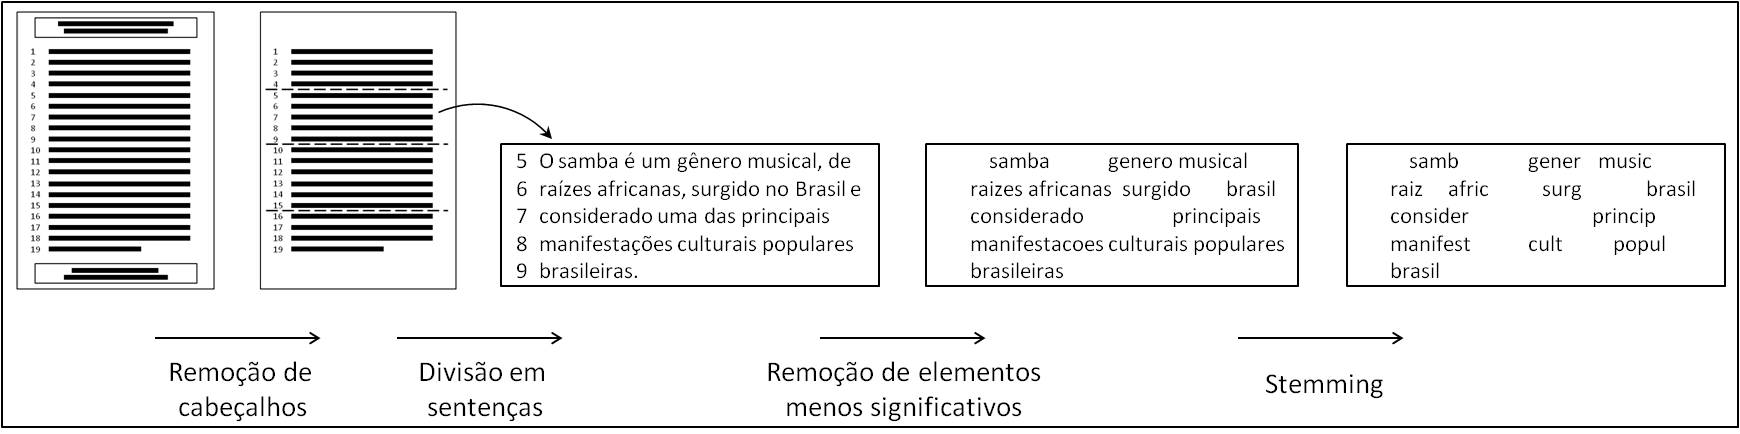
\includegraphics[width=1\textwidth]{conteudo/capitulos/figs/pre-processamento.jpg}
	% \caption{Exemplo de pré-processamento.}
	% \label{fig:exemplopreprocessamento}
% \end{figure}

Entre os primeiros trabalhos voltados a segmentação textual, da literatura 

Entre os principais trabalhos da literatura podemos citar o \textit{TextTiling} ~\cite{Hearst1994} e o \textit{C99}~\cite{Choi2000} são considerados um dos primeiros mais influentes sendo utilizados com \textiit{base lines} em trabalhos recentes.


% Entre os principais trabalhos da literatura podemos citar o \textit{TextTiling} ~\cite{Hearst1994} e o \textit{C99}~\cite{Choi2000}.
% 
% ------   TextTiling
% O \textit{TextTiling} é um algoritmo baseado em janelas deslizantes, em  que, para cada candidato a limite, analisa-se o texto circundante. Um limite ou quebra de segmento é identificado sempre que a similaridade estiver abaixo de um limiar. Possui baixa complexidade computacional e acurácia semelhante a algoritmos mais complexos baseados em matrizes de similaridade como o \textit{C99}.

% Para cada posição candidata o \textit{TextTiling} constrói 2 blocos, um contendo sentenças que a precedem e outro com as que a sucedem. O tamanho desses blocos é um parâmetro a ser fornecido ao algoritmo e determina o tamanho mínimo de um segmento.

% ------   C99
% O \textit{C99} usa matrizes de \textit{rakings} de similaridades e técnicas de \textit{clustering} para encontrar os limites entre os segmentos. Oferece resultados melhores que algoritmos baseados em janelas deslizantes ao custo de maior complexidade computacional.

% Inicialmente é construída uma matriz que contém as similaridades de todas as unidades de texto. Em seguida, essa é transformada substituindo-se cada elemento da matriz original pelo número de elementos vizinhos com similaridade inferior.  Finalmente, utiliza um método de \textit{clustering} % baseado no algoritmo de maximização de Reynar % ~\cite{Reynar1998} 
% para identificar os limites entre os segmentos. 



% ----------------------------------------------------------------------------- 


% usando um conjunto de documentos e uma segmentação manual fornecida por participantes das reuniões. 


% explicar o qe o segmentador faz --> encontrar limites







% Nesse trabalho, escolheu-se o algoritmo \textit{C99} por apresentar resultados satisfatórios e ligeira superioridade em relação ao \textit{TextTiling}. 

% como pode ser visto na Tabela~\ref{tab:configfinal}. 


% O algoritmo \textit{C99} obteve melhor desempenho em acurácia, precisão, $F^1$, $P_k$ e \textit{WindowDiff}, enquanto o \textit{TextTiling} obteve o melhor desempenho em revocação como pode ser visto na Tabela~\ref{tab:configfinal}. 


% \begin{table}[!h]
	% \centering

	% \begin{tabular}{|l|l|c|c|c|c|c|} \hline
		% \textbf{Algoritmo} & 
		% \textbf{Medida} & 
		% \textbf{Média}\\	\hline

	% \textit{C99} & P$_k$			   & 0,116 \\ \hline
	% \textit{C99} & \textit{WindowDiff} & 0,390 \\ \hline
	% \textit{C99} & Acurácia			   & 0,609 \\ \hline
	% \textit{C99} & Precisão			   & 0,720 \\ \hline
	% \textit{C99} & F$^1$			   & 0,655 \\ \hline
	% \textit{TextTiling} &	Revocação  & 0,917 \\ \hline

	% \end{tabular}
	
	% \caption{Melhores resultados obtidos.}
	% \label{tab:configfinal}
% \end{table}


